\documentclass[xcolor=dvipsnames, pdf]{beamer}
\usepackage[spanish]{babel}
\usepackage[utf8]{inputenc}
\usepackage{graphics}
\usepackage{listings}
\mode<presentation>{}
\usecolortheme[named=Orange]{structure}
\usetheme{Copenhagen}
\setbeamertemplate{footline}[frame number]
\setbeamertemplate{navigation symbols}{}
\setbeamertemplate{items}[circle]

\title[Migrando a GNU/Linux]{¿Cómo migrar a GNU/Linux y no morir en el intento?}
\author[VengadoraVG]{Ruth García}
\date[Noviemebre, 2013]{11 de noviembre de 2013}

\AtBeginSubsection[]
{
  \setbeamertemplate{items}[circle]
  \begin{frame}{Esqueleto}
    \tableofcontents[currentsubsection]
  \end{frame}
}

\begin{document}

\begin{section}
  {}  
  \begin{frame}[clean]
    \titlepage
    
\includegraphics[width=2cm]{../img/tux.png}\hfill 
    \scalebox{-1}[1]{
\includegraphics[width=2.5cm]{../img/gnu.png}}
  \end{frame}
\end{section}

\begin{section}
  {¿Quiero?}
  
  \begin{subsection}
    {No es sólo un Sistema Operativo más. Implica...}
    \begin{frame}
      {Libertad}
      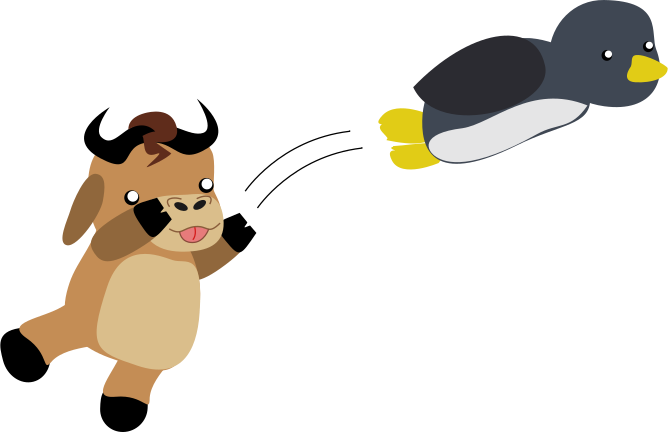
\includegraphics[width=10cm]{../img/libertad.png}
    \end{frame}
    
    \begin{frame}
      {Escalabilidad}
      
\includegraphics[width=10cm]{../img/escalabilidad.png}
    \end{frame}
    
    \begin{frame}
      {Conocimiento}
      
\includegraphics[width=10cm]{../img/conocimiento.png}
    \end{frame}
    
    \begin{frame}
      {Cooperación}
      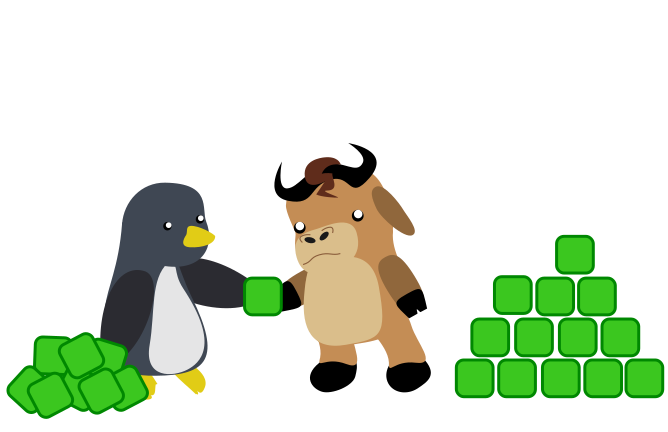
\includegraphics[width=10cm]{../img/cooperacion.png}
    \end{frame}
  \end{subsection}
  
  \begin{frame}
    \vfill
    NO SE TRATA DEL SOFTWARE...  
    \begin{center} SE TRATA DE LAS PERSONAS... \end{center}
    \hfill ¡DE COMPARTIR!
    \vfill
  \end{frame}
  
  \begin{subsection}
    {y en la otra esquina tenemos al... Software Privativo}
    
    \begin{frame}
      {No te deja ver como lo hace}
      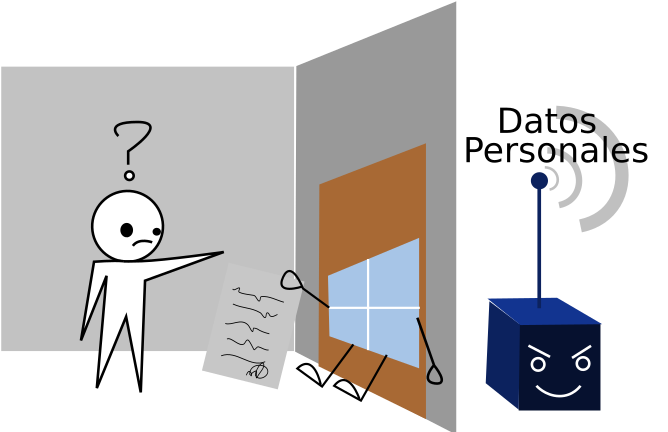
\includegraphics[width=10cm]{../img/evilbox.png}
    \end{frame}

    \begin{frame}
      {Te enga\~{n}a}
      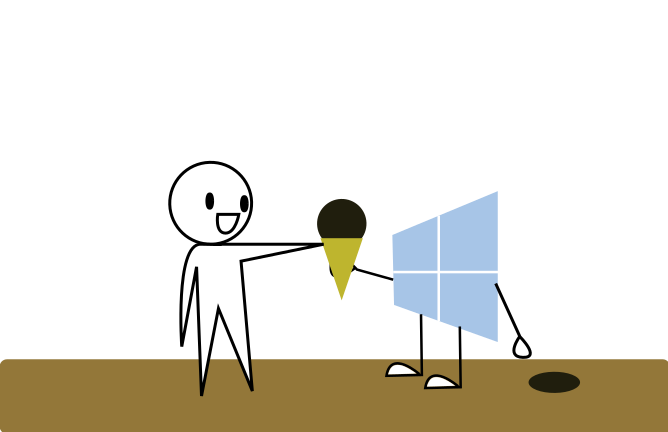
\includegraphics[width=10cm]{../img/secreto.png}
    \end{frame}

    \begin{frame}
      {Te vuelve dependiente}
      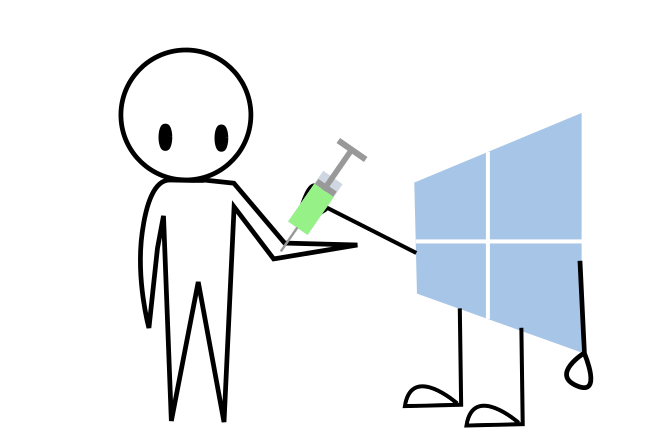
\includegraphics[width=10cm]{../img/judio.png}
    \end{frame}
  \end{subsection}
\end{section}


\begin{section}
  {¿Puedo?}
  
  \begin{subsection}
    {Actitud}
    
    \begin{frame}
      {Determinación}
      \begin{center}¿puedo? == ¿tengo la ACTITUD necesaria?\end{center}
    \end{frame}

    \begin{frame}
      {Disposición...}
      
      \begin{itemize}
      \item<2,5> de TIEMPO para...          
        \begin{itemize}
        \item<2,5> Leer
        \item<2,5> Comprender
        \item<2,5> Compartir *
        \end{itemize}

      \item<3,5> de PERSISTENCIA para...        
        \begin{itemize}
        \item<3,5> Mejorar
        \item<3,5> Sobreponerse a los fracasos
        \end{itemize}

      \item<4,5> y de un poquito de FE en el Software Libre, porque...

        \begin{itemize}
        \item<4,5> todo es posible: ¡ES LIBRE!
        \end{itemize}
      \end{itemize}
    \end{frame}
  \end{subsection}
\end{section}


\begin{section}
  {¡Quiero y puedo!}
  
  \begin{subsection}
    {¡Antes de purgar!}
    \begin{frame}
      {El hardware}
      
      \begin{itemize}
      \item investiga tu hardware en internet:
        
        \begin{itemize}
        \item drivers problematicos
        \item ¡LA TARJETA DE VIDEO!
        \item personas con tu mismo hardware usando GNU/Linux
        \end{itemize}
      \end{itemize}
      ¿404?          
      \begin{itemize}
      \item \textbf{¡Comparte tu experiencia!}
      \end{itemize}
      
    \end{frame}
    
    \begin{frame}        
      \begin{center}Elije tu Distro :D\end{center}
    \end{frame}
    
    \begin{frame}
      {Debian...}            
      \begin{center} 
        \includegraphics[width=11cm]{../img/distros-map/Debian_distro-map.png}
      \end{center}
    \end{frame}
    
    \begin{frame}
      {Debian releases...}
      
      \begin{figure}
        
\includegraphics[width=3cm]{../img/debrelease/squeeze.jpg}
        \\*Debian ``squeeze'' \\*oldstable
      \end{figure}
      
    \end{frame}
    
    \begin{frame}
      {Debian releases...}
      
      \begin{figure}
        
\includegraphics[width=3cm]{../img/debrelease/jessie.jpg}
        \\*Debian ``Jessie'' \\*testing
      \end{figure}
      
    \end{frame}
    
    \begin{frame}
      {Debian releases...}
      
      \begin{figure}
        
\includegraphics[width=3cm]{../img/debrelease/sid.jpg}
        \\*Debian ``Sid'' \\*unstable
      \end{figure}
      
    \end{frame}
    
    \begin{frame}
      {redhat...}
      
      \begin{center} 
        \includegraphics[width=8cm]{../img/distros-map/redhat_distro-map.png} 
      \end{center}
    \end{frame}
  \end{subsection}
  
  \begin{subsection}
    {Instalando aplicaciones}
    
    \begin{frame}
      {¡es fácil con aptitude!}
      
      \begin{itemize}
      \item \texttt{\#{} apt-get install nombre-de-la-aplicacion}
      \item Synaptic
      \end{itemize}
    \end{frame}
    
    \begin{frame}
      {Pero sin aptitude...}
      
      También es fácil XD
      
      \begin{itemize}
      \item Sigue el tutorial de instalación
      \item Si algun paso da un error: investiga \alert{(pero no procedas)}
      \item Si no entiendes: pregunta
      \item y si entiendes: Arregla y \textbf{comparte}
      \end{itemize}
      \pause
      y eso aplica para: \color[rgb]{0.8,0.3,0.3} DRIVERS,
      \color[rgb]{0.3,0.8,0.3} APLICACIONES, 
      \color[rgb]{0.3,0.3,0.8} y, prácticamente todo lo demás :D
    \end{frame}
    
    \begin{frame}
      {Ejecutando un .exe}
      \begin{center}
        \scalebox{-1}[1]{
\includegraphics[width=4cm]{../img/WINE-Logo.png}}
      \end{center}
    \end{frame}
  \end{subsection}
  
  \begin{subsection}
    {¿y qué hay para los devs?}
    
    \begin{frame}
      {Editores de Texto alucinantes \texttt{*u*}}
      como...
      \begin{itemize}
      \item emacs: elisp lo hace poderosamente extensible
      \item vim: sus hotkeys son cortitos :3 
      \item ...
      \end{itemize}
    \end{frame}
    
    \begin{frame}
      {Compatibilidad con Git}
      
      \begin{itemize}
      \item Desde la consola
      \item Instalable desde los repositorios
      \item Offline
      \item Online (como Github)
      \end{itemize}
    \end{frame}
    
    \begin{frame}
      {Repositorio de aplicaciones LIBRES}
      \begin{itemize}
      \item Juegos
      \item IDEs
      \item Cosas raras
      \item ...
      \end{itemize}  
    \end{frame}
    
    \begin{frame}
      {es LIBRE}
      
      \begin{itemize}
      \item podemos \alert{aprender} de su código fuente
      \item podemos \alert{modificar} su código fuente
      \item y podemos \alert{compartirlo y contribuir}
      \end{itemize}
    \end{frame}
    
  \end{subsection}
\end{section}

\begin{section}
  {}
  \begin{frame}[clean]
    {GRACIAS :D}
    \begin{center}
      
\includegraphics[width=4cm]{../img/tux_bye.png}
      \hfill 
\includegraphics[width=4cm]{../img/gnu_bye.png}
      \\Todo el contenido de esta presentación (excepto, talvez, por los
      personajes de Toy Story) es completamente libre \^{} w \^{}
    \end{center}
  \end{frame}    
\end{section}
\end{document}
